\documentclass[12pt]{article}
\usepackage{scrextend}
\usepackage[utf8]{inputenc}
\usepackage[polish]{babel}
\usepackage[T1]{fontenc}%polskie znaki
\usepackage[utf8]{inputenc}%polskie znaki
\usepackage{geometry}
\usepackage{float}
\usepackage{enumitem}
\usepackage{hyperref}
\usepackage{graphicx}
\usepackage{amsmath}

\renewcommand{\baselinestretch}{1.5}


\begin{document}

\begin{flushleft}
    Damian Koper \textbf{241292} \\
\end{flushleft}
\vspace{1cm}
{
    \centering
    {\Huge\scshape\bfseries Modelowanie i analiza systemów informatycznych }\\
    \large{Sieci Petriego - konstrukcja sieci Petriego z łukami hamującymi (cz. 1)}\\
    \vspace{0.5cm}
}
\newcounter{ex}
\setcounter{ex}{0}
\newcommand{\ex}[1]{
    \refstepcounter{ex}{
        \noindent\normalfont\Large\bfseries Zadanie \arabic{ex}.
    } \\
    #1
}

\ex{Rozbudowa sieci}
\vspace{-0.5cm}

\begin{figure}[H]
    \centering
    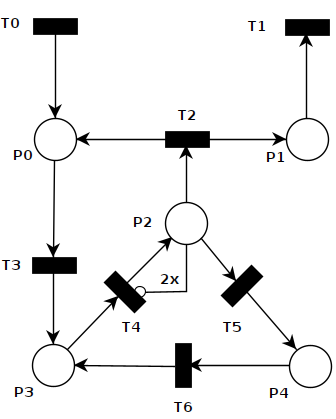
\includegraphics[width=0.5\linewidth]{../../lab7/ex_1}
    \caption{Pojemność miejsca $p_2$ ograniczona do 2 przez łuk hamujący o wadze 2}
\end{figure}

\clearpage

\ex{Rozbudowa sieci}

\begin{figure}[h]
    \centering
    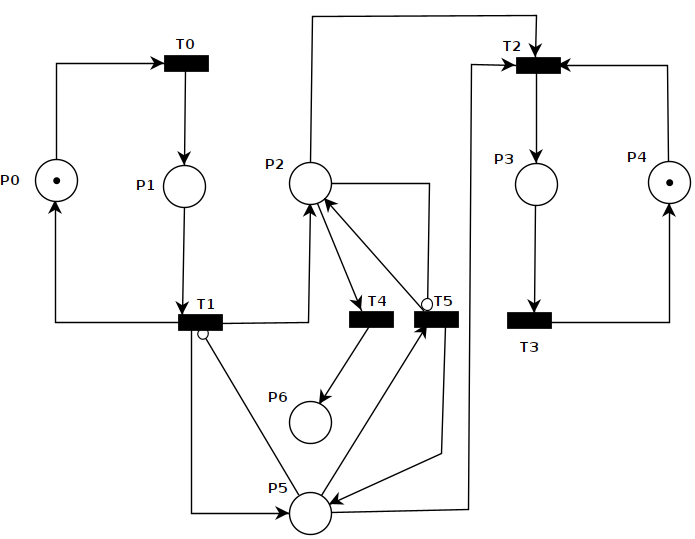
\includegraphics[width=0.7\linewidth]{../../lab7/ex_2}
    \caption{Sieć rozbudowana o obsługę zgubienia i odzyskania wiadomości}
\end{figure}
Dodane i zmodyfikowane elementy:
\begin{itemize}
    \item $p_5$ -- kopia zapasowa wysyłanej wiadomości.
    \item $p_6$ -- zgubione wiadomości.
    \item $t_1$ -- zdarzenie wysłania wiadomości i utworzenie kopii zapasowej w $p_5$, nie można wysłać wiadomości jeśli istnieje kopia zapasowa poprzedniej - wiadomość nie została dostarczona.
    \item $t_2$ -- zdarzenie odebrania wiadomości przez nadawcę razem z usunięciem kopii zapasowej.
    \item $t_4$ -- zdarzenie zgubienia wiadomości.
    \item $t_5$ -- zdarzenie wysłania wiadomości z kopii zapasowej. Kopia zapasowa zostaje zachowana. Nie można wysłać wiadomości jeśli wiadomość jest już w drodze.
\end{itemize}

\end{document}